\section{Laboratory work implementation}

\subsection{Tasks and Points}

\begin{enumerate}

	\item  Initializarea unui nou repositoriu
	\item  Configurarea VCS
	\item  Crearea branch-urilor (cel putin 2)
	\item  Commit pe ambele branch-uri(cel putin 1 commit per branch)
	\item  Setarea unui branch to track a remote origin pe care sa se faca push(GitHub)
	\item  Resetarea unui branch la commit-ul anterior
	\item  Salvarea temporara a schimbarilor care nu se vor face commit imediat
	\item  Folosirea fisierului .gitignore
	\item  Merge 2 branches
	\item  Rezolvarea conflictelor a 2 branches
	\item  Folosirea tag-urilor pentru marcarile semnificative
	
\end{enumerate}

\subsection{Analiza lucrarii de laborator}

Click on \href{https://github.com/OctavianCoroletchiTI154/MIDPS.git}{"Link"} or copy \url{https://github.com/OctavianCoroletchiTI154/MIDPS.git} pentru repozitoriul meu.
\par Task a: \\
Pentru inceput, mi-am facut cont pe github.com. Mi-am creat repozitoriul meu(vezi imaginea a) public. Apoi am facut download la clientul Git.
\par Task b: \\
Mi-am configurat repozitoriul meu, generindu-mi o cheie publica cu ajutorul comenzii $ssh-keygen -t rsa -b 4096 -C  "your email@example.com"$. Apoi mi-am adaugat cheia mea publica la contul meu.Dupa mi-am clonat repozitoriul meu pe masina mea locala cu ajutorul comenzii $"git clone 'repozitoriul meu' "$.\\
\par Task c:\\
Am creat branch-uri cu ajutorul comenzii $"git branch <noul meu branch> "$. (vezi imaginea c). Apoi i-am dat push pe github, cu comanda git push origin lab1.(vezi imaginea c-1).
\par Task d:\\
Am facut commit pe branchurile create cu ajutorul comenzii $git commit -m "name"$. (vezi imaginea d).
\par Task e:\\
Am setat branch-ul lab1, pentru a urmari remote origin pe care sa facem push. Am folosit comanda $git branch -u origin/lab1$ (vezi imaginea e)
\par Task f:\\
Am eliminat branch-ul lab1 din origin cu comanda $git push origin :lab1 $. Apoi am readus lab1 la comitul care avem nevoie.
$git reset --hard 'hashid' $. Apoi am facut push din nou. $git push origin lab1 $. (pentru toate vezi imaginea f)
\par Task g:\\
Am salvat schimbarile temporare cu ajutorul Stash-ului. Aceasta permite salvarea temporara a unor modificari pentru care nu avem nevoie sa facem commit. Se foloseste comanda $ git stash $. Dupa ce se salveaza comenzile modificate, ne putem reintoarce in orice moment spre salvari cu comanda $ git stash apply stash@{0} $, sau in loc de stash@{0} cu id-ul salvat. Pentru a vedea intreaga lista de stash-uri, folosim $ git stash list $. (vezi imaginea g).
\par Task h:\\
.gitignore, este un fisier, in care specificam ce tipuri ce file-uri nu dorim sa fie prezente in repozitoriul nostru Git. In imaginea raspunzatoare de task-ul h, se va observa fisierul nostr .gitignore si tipurile de fisiere ce vor fi ignorate. (vezi imaginea h).
\par Task i:\\
Ajungind la un moment, cind modificarile pentru un anumit branch ajung la un statut final, atunci putem sa imbinam branch-ul aditional cu cel principal. Pentru inceput, ne schimbam pe branch-ul principal cu comanda $ git checkout master $ , apoi le imbinam cu comanda $ git merge lab1 $ unde master si lab1, sunt branch-uri. Apoi putem face delete pentru branch-ul adition lab1, pentru ca nu mai avem nevoie de el cu comanda $ git branch -d lab1 $. (vezi imaginea i pentru implementari).
\par Task j:\\
Conflictele apar atunci cind incerci sa faci merge la 2 branchu-uri, in care in ambele au loc modificari in acelasi fisiel. Cum ar fi situatia intilnita de mine, in care 2 branch-uri, aveau modificari diferite in README.md. Conflictul intilnit (vezi imaginea j). Apoi trebuia sa decid ce schimbari doresc sa pastrez pentru a continua peste conflict. (vezi j-1). Dupa aia, totul a continuat cu succes.
\par Task k:\\
Tagurile sunt folosite pentru a marca anumite evenimente importante din modificari.Ele se implementeaza cu ajutorul comenzii $ git tag -a 'name' -m "description" $. 
Dupa se da push pentru a vedea si altii tagurile noastre. (vezi imaginea k, pentru implementare). 
\clearpage

\subsection{Imagini}
\begin{center}
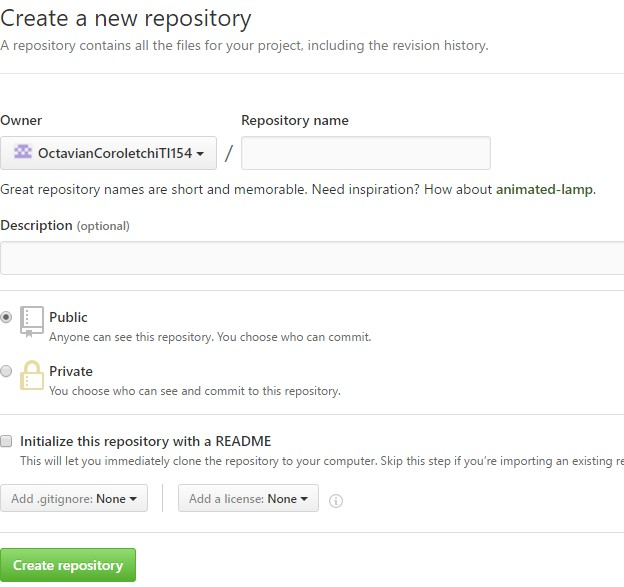
\includegraphics[scale=0.5]{a} \\ 
Imaginea - "a" \\
\vspace{10 mm}
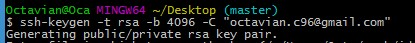
\includegraphics[scale=1]{b} \\
Imaginea - "b" \\
\vspace{10 mm}
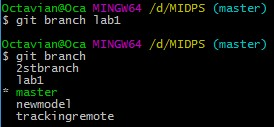
\includegraphics[scale=1]{c} \\
Imaginea - "c" \\
\vspace{10 mm}
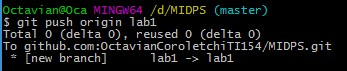
\includegraphics[scale=1]{c-1} \\
Imaginea - "c-1" \\
\vspace{10 mm}
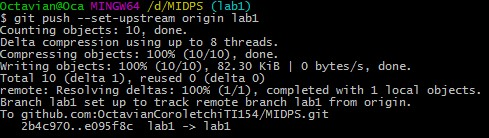
\includegraphics[scale=1]{d} \\
Imaginea - "d" \\
\vspace{10 mm}
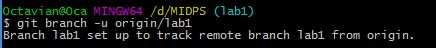
\includegraphics[scale=1]{e} \\ 
Imaginea - "e" \\
\vspace{10 mm}
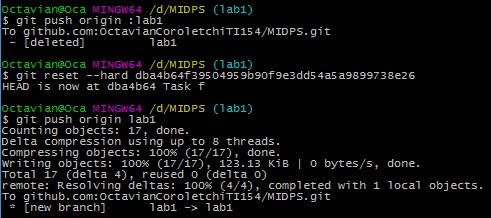
\includegraphics[scale=1]{f} \\ 
Imaginea - "f" \\
\vspace{10 mm}
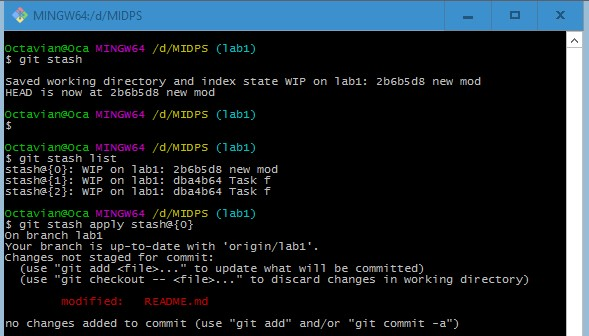
\includegraphics[scale=1]{g} \\
Imaginea - "g" \\
\vspace{10 mm}
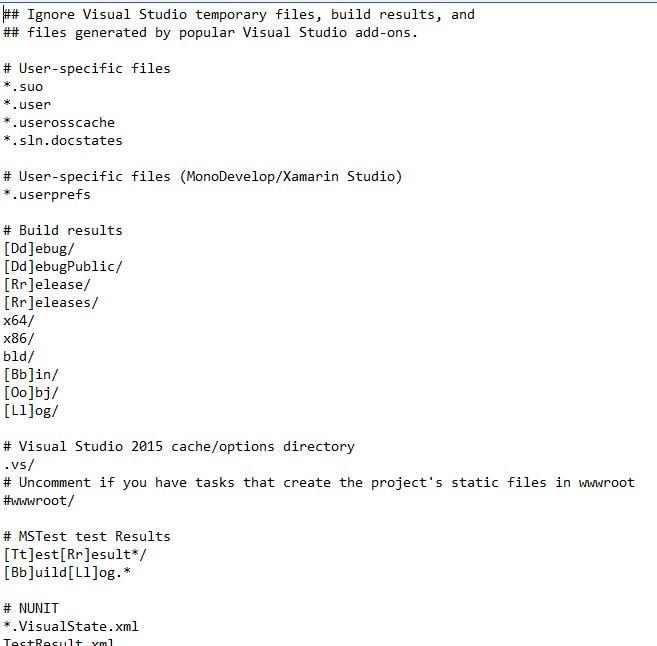
\includegraphics[scale=1]{h} \\
Imaginea - "h" \\
\vspace{10 mm}
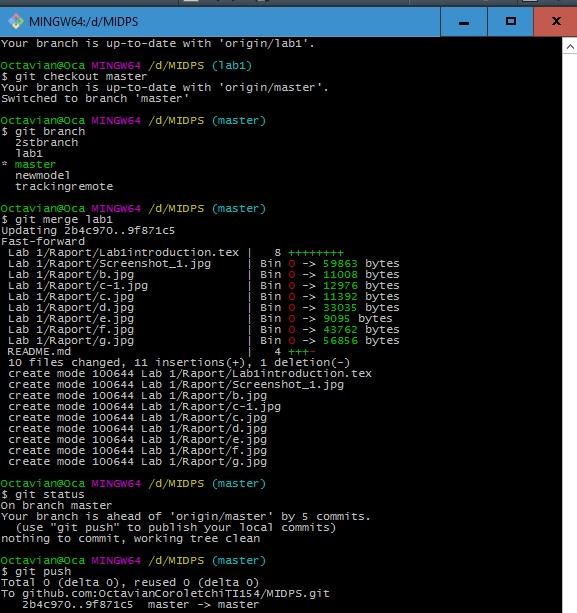
\includegraphics[scale=0.9]{i} \\ 
Imaginea - "i" \\
\vspace{10 mm}
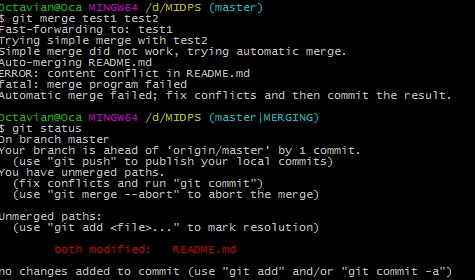
\includegraphics[scale=1]{j} \\
Imaginea - "j" \\
\vspace{10 mm}
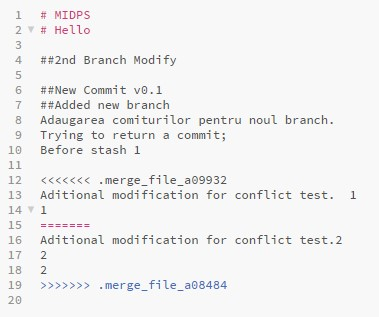
\includegraphics[scale=1]{j-1} \\
Imaginea - "j-1" \\
\vspace{10 mm}
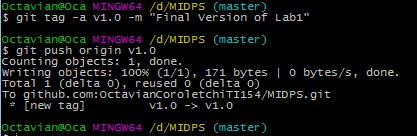
\includegraphics[scale=1]{k}\\
Imaginea - "k" \\
\vspace{10 mm}
\end{center}


